\documentclass[a4paper,12pt]{article}
\usepackage{graphicx}

\usepackage{epstopdf}
\usepackage{gensymb}
\usepackage{float}
\usepackage{mathtools}
\usepackage{setspace}
\usepackage{tabularx}
%% Definitioner för LIPS-dokument

\usepackage[swedish]{babel}
\usepackage[utf8]{inputenc}
\usepackage[T1]{fontenc}
\usepackage{times}
\usepackage{ifthen}
\usepackage[labelfont=it]{caption}

\usepackage[margin=25mm]{geometry}

\def\arraystretch{1.6}

\usepackage{fancyhdr}
\pagestyle{fancy}
\lhead{}
\chead{\LIPSprojekttitel}
\rhead{\LIPSdatum}
\lfoot{\LIPSkursnamn \\ \LIPSdokumentansvarig}
\rfoot{\LIPSprojektgrupp \\ \LIPSgruppepost}

\setlength{\parindent}{0pt}
\setlength{\parskip}{1ex plus 0.5ex minus 0.2ex}


\newcommand{\twodigit}[1]{\ifthenelse{#1<10}{0}{}{#1}}
\newcommand{\dagensdatum}{\number\year-\twodigit{\number\month}-\twodigit{\number\day}}

%% ------------------------------------------
% NYBILD
% Skapar centrerad bild med caption
%   
% #1: Filens url relativt '/bilder/'
% #2:  Caption
% #3: Label
% #4: Skalning i förhållande till textwidth
%% ------------------------------------------
\newcommand{\nyBild}[4] 
{\begin{figure}[H]
  \centering
 \emph{\includegraphics[angle=0,width=#4\textwidth]{bilder/#1}}
  \caption{\emph{#2}}
  \label{fig:#3}
\end{figure}}

%%  Redefinitions of commands containing @
\makeatletter
\makeatother

\newcommand{\LIPStitelsida}{%
{\ }\vspace{45mm}
\begin{center}
  \textbf{\Huge {\sffamily \LIPSdokumenttyp}}
\end{center}
\begin{center}
  {\Large \LIPSredaktor}
\end{center}
%\begin{center}
%  {\Large Version \LIPSversion}
%\end{center}
\vspace{60mm}
%\begin{center}
%  {\large Status}\\[1.5ex]
%  \begin{tabular}{|*{3}{p{40mm}|}}
%    \hline
%    Granskad & \LIPSgranskare & \LIPSgranskatdatum \\
%    \hline
%    Godkänd & \LIPSgodkannare & \LIPSgodkantdatum \\
%    \hline
%  \end{tabular}
%\end{center}
\newpage
}


\newenvironment{LIPSprojektidentitet}{%
{\ }\vspace{45mm}
\begin{center}
  {\Large PROJEKTIDENTITET}\\[0.5ex]
  {\small
  \LIPSprojektgrupp, \LIPSartaltermin, \LIPSprojekttitel\\
  Tekniska högskolan vid Linköpings universitet, ISY
  }
\end{center}
\begin{center}
  \begin{tabular}{|l|p{45mm}|p{25mm}|l|}
    \hline
    \textbf{Namn} & \textbf{Ansvar} & \textbf{Telefon} & \textbf{E-post} \\
    \hline
}
{
    \hline
  \end{tabular}
\end{center}
\begin{center}
  {\small
    \textbf{E-postlista för hela gruppen}: \LIPSgruppepost\\
    \textbf{Kontaktperson hos kund}: \LIPSkundkontakt\\
    \textbf{Kursansvarig}: \LIPSkursansvarig\\
    \textbf{Handledare}: \LIPShandledare\\
  }
\end{center}
\newpage
}
\newcommand{\LIPSgruppmedlem}[4]{\hline {#1} & {#2} & {#3} & {#4} \\}



\newenvironment{LIPSdokumenthistorik}{%
\begin{center}
  Dokumenthistorik\\[1ex]
  \begin{small}
    \begin{tabular}{|l|l|p{60mm}|l|l|}
      \hline
      \textbf{Version} & \textbf{Datum} & \textbf{Utförda förändringar} & \textbf{Utförda av} & \textbf{Granskad} \\
      }%
    {%
      \hline
    \end{tabular}
  \end{small}
\end{center}
}
\newcommand{\LIPSversionsinfo}[5]{\hline {#1} & {#2} & {#3} & {#4} & {#5} \\}



\newenvironment{packed_itemize}{
\begin{itemize}
	\setlength{\itemsep}{1pt}
    \setlength{\parskip}{0pt}
    \setlength{\parsep}{0pt}
}{\end{itemize}}

\newenvironment{packed_enumerate}{
\begin{enumerate}
	\setlength{\itemsep}{1pt}
    \setlength{\parskip}{0pt}
    \setlength{\parsep}{0pt}
}{\end{enumerate}}





%%% Local Variables: 
%%% mode: latex
%%% TeX-master: "kravspec_mall"
%%% End:

\usepackage{sectsty}
\allsectionsfont{\sffamily}

\frenchspacing

\renewcommand{\thepage}{\roman{page}}

\newcommand{\LIPSartaltermin}{VT14}
\newcommand{\LIPSkursnamn}{TSEA56 Elektronik kandiatprojekt}

\newcommand{\LIPSprojekttitel}{Lagerrobot}

\newcommand{\LIPSprojektgrupp}{Grupp 1}
\newcommand{\LIPSgruppepost}{tsea56-2014-grupp-1@googlegroups.com}
\newcommand{\LIPSdokumentansvarig}{LIPS Designspecifikation}

\newcommand{\LIPSkund}{ISY, Linköpings universitet, 581\,83 Linköping}
\newcommand{\LIPSkundkontakt}{Tomas Svensson, 013-28 13 68, tomass@isy.liu.se}
\newcommand{\LIPSkursansvarig}{Tomas Svensson, 013-28 13 68, 3B:528, tomass@isy.liu.se}
\newcommand{\LIPShandledare}{Anders Nilsson, 3B:512, 013-28 26 35, anders.p.nilsson@liu.se}


\newcommand{\LIPSdokumenttyp}{Designspecifikation}
\newcommand{\LIPSredaktor}{Patrik Nyberg}
\newcommand{\LIPSversion}{0.1}
\newcommand{\LIPSdatum}{\dagensdatum}

\newcommand{\LIPSgranskare}{}
\newcommand{\LIPSgranskatdatum}{}
\newcommand{\LIPSgodkannare}{}
\newcommand{\LIPSgodkantdatum}{}

\begin{document}

\LIPStitelsida

%% Argument till \LIPSgruppmedlem: namn, roll i gruppen, telefonnummer, epost
\begin{LIPSprojektidentitet}
  \LIPSgruppmedlem{Karl Linderhed}{Projektledare (PL)}{073-679 59 59}{karli315@student.liu.se}
  \LIPSgruppmedlem{Patrik Nyberg}{Dokumentansvarig (DOK)}{073 -049 59 90}{patny205@student.liu.se}
  \LIPSgruppmedlem{Johan Lind}{}{070-897 58 24}{johli887@student.liu.se}
  \LIPSgruppmedlem{Erik Nybom}{}{070-022 47 85}{johjo939@student.liu.se}
  \LIPSgruppmedlem{Andreas Runfalk}{}{070-564 23 79}{andru411@student.liu.se}
  \LIPSgruppmedlem{Philip Nilsson}{}{073-528 48 86}{phini326@student.liu.se}
  \LIPSgruppmedlem{Lucas Nilsson}{}{073-059 42 94}{lucni395@student.liu.se}
\end{LIPSprojektidentitet}


\renewcommand*\contentsname{Innehåll}
\begin{spacing}{0.5}
\tableofcontents{}
\end{spacing}
\newpage

%% Argument till \LIPSversionsinfo: versionsnummer, datum, ändringar, utfört av, granskat av
%\addcontentsline{toc}{section}{Dokumenthistorik}
\begin{LIPSdokumenthistorik}
  \LIPSversionsinfo{0.1}{2014-03-08}{Första utkast.}{PaN}{}
  %\LIPSversionsinfo{1.0}{2012-02-14}{Första utkast.}{}{}
\end{LIPSdokumenthistorik}
\newpage

\renewcommand{\thepage}{\arabic{page}}
\setcounter{page}{1}

\section{Systemöversikt}
\nyBild{Figur__versikt_systemet.jpg}{Schematisk beskrivning av systemet}{systemschema}{1}

Roboten ska vara uppbyggd av fyra olika delsystem (chassi, sensor, arm och kommunikation) som vart och ett har sin specifika uppgift att sköta. Målet är att ett delsystem inte ska behöva känna till hur de andra delsystemen fungerar och man ska kunna byta ut ett delsystem mot en annan implementation utan att behöva ändra på övriga delsystem. Förutom robotens fyra delsystem kommer också en programvara till en dator att utvecklas för övervakning och styrning. Den kommer att både kunna operera i ett fjärrstyrt och i ett autonomt läge. I första hand ska autonomin endast innefatta linjeföljning och några förutbestämda armrörelser (t.ex. arm ut, arm in, lämna av föremål åt höger). Om det finns tid i projektet kommer autonom lokalisering och upplockning av föremål också implementeras.

Sensorenheten ska kontinuerligt övervaka de olika sensorerna roboten har och omvandla dess primärdata till systemanvändbara enheter för att sedan kunna skicka dessa vidare till andra delsystem.

Kommunikationsenheten ska fungera som en förbindelselänk mellan omvärlden och roboten. Den ska kunna bli tillfrågad och skicka bekräftelse om de beslut som roboten gör samt status över de olika delsystemen och omgivningsobservationer.

Chassienheten fungerar som det handlingsbeslutande organet på roboten. Den ska vid automatiskt läge vet hur roboten ska agera vid olika situationer. Den styr också hjulen på roboten, det vill säga att den genom sensordata och reglering beräknar hastighet på hjulen för att kunna svänga och hålla kursen längst banan.

Armenheten ska vid en avhämtningsstation, utifrån identifiering av var ett objekt befinner sig, kunna plocka upp detta med robotarmen som är monterad på chassit. Det kommer ha kontroll över samtliga servon och vet hur dessa ska röras vid kommando. Med hjälp av invers kinematik ska den kunna, vid automatiskt läge, beräkna hur vardera led skall röra sig för nå objektet och för att plocka upp det.

PC-programvaran ska visa upp ett instrumentbräde på för användaren att både se robotens beslut samt statusinformation. Här ska också roboten kunna styras med olika sorters kommandon som finns.

\subsection{Sensorer och sensorplacering}

En linjesensor ska sitta längst fram på roboten, nära marken. En RFID-läsare ska sitta parallellt med marken under roboten, då den endast har 7~cm läsavstånd till taggarna som ligger på marken. På vardera sida av roboten kommer en avståndssensor sitta placerad på ett servo, för att skanna efter objekt att plocka upp. På armen kommer det också att sitta avståndssensor för att kunna hitta och plocka upp objekt.

\section{Kommunikationsenhet}
Kommunikationsenheten är robotens gränssnitt för interaktion med omvärlden och har två uppgifter. Den ska
\begin{itemize}
\item agera som ett gränssnitt mot LCD-skärmen och möjliggöra att alla delsystem kan skriva ut information på den.
\item hantera den seriella kommunikationen över blåtand och möjliggöra att roboten kan skicka och ta emot information till och från PC-gränssnittet.
\end{itemize}

Figur \ref{fig:kommblock} ger en övergripande bild över kommunikationsenhetens beståndsdelar.

\nyBild{Block-komm.png}{Blockschema över kommunikationsenheten.}{kommblock}{0.9}

\subsection{LCD-gränssnitt}
LCD-skärmen som är monterad på kommunikationsenheten är av modellen JM162A. Den styrs genom en parallell databuss och ett antal styrsignaler från kommunikationsenhetens processor till en intern processor i LCD-enheten. Skärmen har två rader med 16 tecken vardera. \cite{lcd}

Information skickas till LCD-enheten antingen som instruktioner eller data. Styrsignalernas koppling visas i figur \ref{fig:kommblock}. \verb|RS| styr om databussens värde tolkas som instruktion eller data, \verb|R/W| styr ifall information ska skrivas eller läsas, och styrsignalen \verb|E| aktiverar överföring av information. Genom att låta \verb|E| gå från hög till låg läser LCD-enheten in värdet som finns på databussen, antingen som en instruktion som ska utföras (om \verb|RS| är låg) eller som data som ska lagras i LCD-enhetens minne (om \verb|RS| är hög). Figur \ref{fig:lcdinit} visar vilka kommandon som skickas för att initiera LCD-enheten.

\nyBild{lcd-init.png}{Flödesschema över initialisering av LCD-enhet. Kommandon som skickas är kursiverade och har värdena på DB (i binär notation), RS och R/W som parametrar.}{lcdinit}{0.4}

Efter denna initiering kan data skrivas ut på skärmen genom att sätta \verb|RS| till 1 och skriva ut ASCII-koden\footnote{American Standard Code for Information Interchange, ett sätt att koda grundläggande alfanumeriska tecken och andra symboler.} för en symbol på databussen. Genom att först skicka en instruktion för att ställa in vilken adress i dataminnet som ska skrivas till härnäst kan man välja var en symbol ska skrivas ut, en viss adress i dataminnet svarar mot en position på skärmen.

Alla delsystem kan skriva ut information på skärmen genom ett gemensamt bibliotek, \textit{lcd\_interface}, som beskrivs närmare i avsnitt \ref{sec:lcd_interface}.


\subsection{Seriell kommunikation över blåtand}
Anslutningen till datorn sker med blåtandsmodemet \emph{BlueSMiRF Gold} som är monterat på roboten \cite{bluetooth}. På PC-sidan skapas vid parkoppling med modemet en virtuell serieport, som emulerar en fysisk COM-port eller motsvarande. Kommunikationen sker sedan över denna port som om den vore en vanlig RS-232-port\footnote{RS-232 är en typ av seriell kommunikation vid överföring av data \cite{rs232}.}. 

På robotsidan används AVR-processorns inbyggda modul för USART, och det gemensamma biblioteket för USART som används av flera delsystem -- se avsnitt \ref{sec:usart}. Följande parametrar ställs in i det protokoll som roboten använder:
\begin{itemize}
\item Datahastigheten är 115 200 bps.
\item Data skickas som 8-bitars värden utan någon paritetsbit.
\item Ingen flödeshantering eller handskakning används.
\item Varje värde om 8 bitar avslutas med en stoppbit.
\end{itemize}

Hur olika typer av information överförs mellan robot och PC beskrivs närmare i avsnitt \ref{sec:bt-protokoll}.

\section{Sensorenhet}
Sensorenhetens uppgift är att samla in rådata från de olika sensorerna och formatera denna till information som är användbar för robotens övriga delsystem. På begäran av andra delsystem skickar sensorenheten ut data via bussen. Sensorenheten är utrustad
med en linjesensor vars uppgift är att ge information om robotens position i förhållande till tejplinjen. Informationen används som styrdata och skickas över bussen i form av en tyngdpunkt till chassimodulen för styrreglering.

Vidare är roboten utrustad med två sidoskannrar, en på vardera sida. Dessa används för att lokalisera föremålet roboten ska plocka upp. Om ett föremål hittas räknar sensorenheten ut en koordinat för föremålet och skickar koordinaten över bussen till armenheten.


\subsection{Sensorer}
Sensorenheten använder tre olika sensortyper: avståndssensor, linjesensor och RFID-läsare.
Dessa beskrivs kortfattat nedan. En djupare beskrivning av hur komponenterna fungerar finns i bilaga sensorfördjupning.

\subsubsection{Avståndssensorer}
Avståndssensorerna används till robotens sidoskannrar. De mäter avstånd genom att skicka ut infrarött ljus som sedan reflekteras tillbaka i en PSD, Position Sensitive Detector. Avståndssensorerna som används fungerar för avstånd mellan \mbox{$4-30$ cm}. Eftersom de först mäter ett digitalt värde och sedan skickar ut en analog spänning uppstår brus på utsignalen. Detta brus är relativt högfrekvent varför det filtreras bort med hjälp av ett lågpassfilter innan signalen når processorn. Se kopplingsschema, figur \ref{fig:senskoppling}.

En avläsning från en avståndssensor görs genom att omvandla sensorns analoga utspänning till ett digitalt värde. När A/D-omvandlingen är klar jämförs den A/D-omvandlade spänningen med en tabell över kända avstånd och spänningar för att översätta denna till ett avstånd i millimeter. Värden som inte finns i tabellen beräknas med linjärinterpolering. 

Avståndssensorerna är, inom det intervall de är designade att arbeta, kapabla till att uppnå hög precision men olika föremål kan få avståndssensorn att ge ut olika spänningar för samma avstånd. Detta leder till att det är av stor vikt att alla avståndssensorer kalibreras i den miljö de är tänkta att användas. Kalibreringen sker genom att identifiera vilka spänningar som svarar mot kända avstånd och föra in dessa som konstanter i sensorenhetens programkod. Avståndssensorerna har även ett område inom vilket de klarar av att känna av avstånd. Detta område breder huvudsakligen ut sig i horisontell led. Detta har på roboten tagits i beaktning genom att montera de avståndssensorer som sitter på sidoskannrarna vertikalt snarare än horisontellt.

\subsubsection{Linjesensor}
\label{sec:linjesensor}
Reflexsensormodulen består av en uppsättning IR-dioder och fototransistorer som tillsammans används för att mäta reflektionsförmågan hos underlaget. Eftersom reflexsensormodulen består av 11~stycken separata IR-dioder och fototransistorer används en multiplexer och en demultiplexer för att styra sensorn. Demultiplexern driver IR-dioderna och multiplexern används för att ta in insignalerna från fototransistorerna. Linjesensorn är kopplad i enlighet med kopplingsschemat i figur \ref{fig:senskoppling}.

Reflexsensorn ger ut en analog spänning som är omvänt proportionell mot underlagets reflekterande ljusstyrka. En inläsning från linjesensorn sker genom ett funktionsanrop till linjesensorinläsningsfunktionen som finns på sensorenheten. När denna funktion anropas uppdateras en uppsättning variabler som är lagrade i en vektor. Vektorn är 11 element lång, där varje element representerar en reflexsensor.

När uppdateringen av linjesensorn startas för första gången är multiplexrarna som styr linjesensorn inställda så att reflexsensorn längst till vänster väljs. Efter detta startas A/D-omvandling på kanal~0 som svarar mot den pinne på processorn som reflexsensormodulen är kopplad till. Under vidare körning så påbörjas varje uppdatering av reflexsensorerna med att en A/D-omvandling startas varefter programmet väntar på att omvandlingen ska slutföras. När A/D-omvandlingen är färdig läggs sedan det erhållna värdet in i linjesensorns datavektor.


\subsubsection{RFID-läsare}
Den RFID-läsare som används är en “Parallax Serial”. Denna kräver två pinnar på processorn enligt kopplingsschema i figur \ref{fig:senskoppling}. När chassit har stannat på en station beordras sensorenheten att göra en RFID-läsning. Då körs ett program på sensorenheten som aktiverar läsaren, rensar läsarbufferten och sedan väntar programmet på att en inläsning sker, vilket i regel tar cirka 150 - 300 ms. Läsaren kommunicerar med sensorenhetens processor via USART och så fort antennen låst sig på en tagg skickas värdet till processorn där det lagras i en buffert. Så fort det finns data i bufferten väntar programmet ytterligare 50 ms för att all data ska hinna läsas in till bufferten från RFID-taggen innan avläsning av bufferten sker. Sedan jämförs det inlästa värdet med RFID-taggar som redan finns lagrade i processorns minne. Om någon av de redan lagrade taggarna matchar det inlästa värdet skickar sensorenheten tillbaka den siffra som står på motsvarande RFID-tagg. Om ingen inläsning gjorts innan 400 ms ger programmet upp och skickar till chassienheten att inget hittades.

\subsection{Sidoskanner}
Sidoskannerns uppgift är att hitta det objekt som ska plockas upp när roboten har stannat vid en plockstation. Sidoskannern består av två avståndssensorer, på höger respektive vänster sida om roboten, monterade på varsitt servo. Servona styrs med hjälp av pulsbreddsmodulering. Servot får en puls var 20:e~ms och pulsbredden avgör vilket läge servot antar. En pulsbredd på ungefär 0.5~ms motsvarar servots minsta utslag och en pulsbredd på ungefär 2.5~ms motsvarar max vinkelutslag. Värden på dessa utslag varierar dock något från servo till servo.

För att få ett servot att svepa över robotens ena sida ökas pulsbredden inkrementellt med en stegkonstant motsvarande ett servoutslag på en grad. För varje iteration, dvs. för varje vinkel servot står i, kommer avståndssensorn lägga in 20 stycken A/D-omvandlade avståndsmätningar i en array för att sedan ta medianvärdet av mätningarna. Detta görs för att bli av med eventuella avvikande värden som fås ur avståndssensorerna. Slutligen omvandlas värdet till ett avstånd i millimeter genom att interpolera mellan de olika referensvärden som finns lagrade i processorn. Om avståndet är större än vad armens räckvidd är innebär det att att inget föremål detekterats och servots vinkel stegas upp ytterligare en grad. 

När avståndssensorn däremot påträffar ett föremål inom armens räckvidd sparas både vinkeln som servot står i och avståndet till föremålet undan innan sidoskannern stegar upp igen. För varje vinkel som avståndssensorerna fortfarande träffar föremålet sparas avståndet undan och slutligen även den sista vinkeln då den fortfarande träffade ett föremål.

Den vinkel som föremålet slutligen beräknas stå i ligger mitt emellan den första och sista vinkeln där föremålet detekterats. Vidare beräknas avståndet till föremålet som medianen av de mätningar som gjordes under tiden föremålet detekterats. Detta görs för att minimera den inverkan som kraftigt avvikande värden annars skulle kunna få. Medelvinkeln $\alpha$ och medianavståndet $L$ används sedan för att beräkna en koordinat utifrån vilken armen kan plocka upp föremålet. Denna koordinat är planpolär och består således av en vinkel $\beta$ och ett avstånd, $R$. Här är $\beta$ den vinkel som basplattan ska stå i för att armen ska vara riktad mot föremålet och $R$ är avståndet från robotens mittpunkt ut till föremålet. Se figur \ref{fig:sidoskanner}
\nyBild{sidoskanner.png}{Vänster sidoskanner.}{sidoskanner}{0.7}


\subsubsection{Koordinatberäkning}
När sidoskannern har hittat ett objekt och med flera mätningar noggrant identifierat avståndet $L$ och vinkeln $\alpha$ används dessa för att räkna ut $R$ och $\beta$ genom att kalla på två funktioner, \texttt{calculate\_angle\_coordinate} och \texttt{calculate\_distance\_coordinate}.
Vid montering av sidoskannrarna mäts avståndet från robotens origo, dvs. armens mittpunkt, till servonas rotationsaxel, se figur \ref{fig:sidoskanner}. Avståndet definieras som konstanten Origo-to-scanner-distance och används i koordinatberäkningsfunktionerna.

En temporär koordinat för objektet i förhållande till origo bestäms:
$$\begin{pmatrix}
x \\ y
\end{pmatrix}
 = 
\begin{pmatrix}
Konstant+L \sin(\alpha) \\ 
L \cos(\alpha)
\end{pmatrix}$$

Sen fås $R$ och $\beta$:
$$\begin{pmatrix}
R \\ \beta
\end{pmatrix}
 = 
\begin{pmatrix}
\sqrt{x^2 + y^2} \\ 
\arctan(\frac{x}{y})
\end{pmatrix}$$

\subsection{Linjeföljning}
Linjeföljning är en central del i robotens förmåga att utföra sitt uppdrag. Nedan beskrivs de väsentliga delar som ingår i denna process. Inläsning från linjesensorn beskrivs i \ref{sec:linjesensor}.

\subsubsection{Korsning, avbrott och plockstationsdetektering}

Plockstationsdetektering sker genom att roboten först och främst kontrollerar huruvida linjesensorn registrerar tejp utöver den tejpade linjen. Ifall att de fyra sensorerna längst ut antingen till höger eller vänster på reflexsensormodulen indikerar tejp innebär detta att vi antingen är vid en plockstation eller vid en korsning. Först när det har skett 2000 A/D-omvandlingar kommer roboten att stanna på en plockstation. Under denna tid kommer roboten fortlöpande att kontrollera huruvida linjesensorn registrerar tejp på den andra sidan om roboten. På detta sätt säkerställs att roboten inte stannar vid korsningar. Om den å andra sidan registrerar tejp på andra sidan också innebär det korsning och den kan köra vidare. 

För att hantera avbrott i tejplinjen kontrolleras fortlöpande huruvida roboten är över en linje. I det fall att roboten tappar linjen helt och hållet så kommer den utifrån sensorenheten skickade tyngdpunkten att vara 127, vilket motsvarar att linjen ligger på mitten. Eftersom att avbrott i tejpen i enlighet med banspecifikationen som längst får vara 10 centimeter långa är detta tillvägagångssätt fullt tillräckligt för att hantera avbrott i tejpen.
 
%\nyBild{programfl_de-_sensorenheten_uppdaterar_variabler.jpg}{Programflöde för att upptäcka korsning eller plockstation}{senskorsning}{0.8}


\subsubsection{Tyngdpunktsberäkning}
För att roboten ska känna till sin egen position i förhållande till linjen så ses de värden som registreras av de individuella sensorerna på reflexsensorn som tyngder. Ett högre värde motsvarar en större tyngd. De olika tyngder som finns på linjesensorn används sedan för att beräkna en tyngdpunkt hos linjesensorn. Eftersom att de reflexsensorer som läser av tejpen kommer att väga betydligt mer än de som läser av golvet kommer tejpen alltid att finnas där tyngdpunkten beräknas ligga hos linjesensorn.

Tyngdpunktsberäkningen använder sig av två stycken variabler. Den första variabeln innehåller linjesensorns totalvikt, alltså summan av de individuella reflexsensorernas värden. Den andra variabeln innehåller sensorns totalvikt, men där de olika reflexsensorerna även har blivit multiplicerade med en skalfaktor. Denna skalfaktor fyller två funktioner. Först och främst behövs den för att ge sensorerna på kanterna en större hävarm relativt linjesensorns mittpunkt. Vidare används den till att skala den slutgiltiga tyngdpunkten så att hela talområdet hos det åtta bitar stora returvärdet används för att representera linjen. Denna metod kommer att resultera i att tyngdpunkten representeras av ett åtta bitar stort heltalsvärde.

Då tyngdpunkten är 0 ligger tejpen alltså längst till vänster på reflexsensorn på samma sätt som en mekanisk tyngdpunkt hade legat längs till vänster om all massa hos en linje hade legat till vänster. Motsvarande innebär tyngdpunkt 255 att linjen ligger längs ut till höger på linjesensorn.








\section{Chassienhet}
\emph{Det här avsnittet ska innehålla mera detaljerade blockscheman och beskrivningar av modulen.
Tänk på läsbarheten och växla mellan figurer och text.}
\section{Armenhet}

Robotens arm är av modell PhantomX Reactor från Trossen Robotics, som är en servostyrd arm med 4 rotationsleder och en griphand varpå det sitter totalt 7~st AX-12A-servon. Armen kontrolleras av en microprocessor, ATmega 1284, genom att parallellkoppla servona till en seriell UART-port. Kommunikationen till servona sker via half duplex via en tri state buffer. Armen har en maximal räckvidd på 38~cm och en bas med  300~grader rotationsfrihet.

\subsection{Funktion}

Armen kan styras manuellt via PC-programvaran och kan köras i autonomt läge. Enhetens huvudprogram är avvaktande tills dess att kommando skickas till enheten vilket kan antingen vara ett manuellt styrningskommando eller en order från chassienheten att ta hand om upplockning av objekt.

\subsubsection{Manuellt läge} 

Vid manuellt läge får armen ingen upplockningsorder från chassienheten och väntar därför endast efter ett styrkommando från PC. Från PC får den ett kommando att röra sig i en viss riktning i koordinatsystemet visat i figur \ref{fig:arminverskinematik}.

Användaren kan välja att röra armen i djupled (Y-axeln), i höjd (Z-axeln), rotera runt Z-axeln eller öppna och stänga klon. Vid ett styrkommando rör sig armen i den angivna riktningen tills dess att ett kommando om att stanna rörelse i den riktingen ges från PC eller om den nått max-läget. Rörelse görs genom att kontinuerligt beräkna hur vinkeln av vardera led på armen skall ändras för att röra sig ett litet steg i den beordrade riktningen, detta görs genom beräkningar i inverterad kinematik (se \ref{inverskinematik}), sedan gör lederna en vinkelförändring för att sedan repetera enligt ovan.

Armen kan också via PC automatiskt röra sig till ett förbestämt läge, ett startläge, där rörelsen även här beräknas med inverterad kinematik till den position som startläget har. Först rör sig armen rakt upp från det nuvarande läget för att sedan röra sig till den position som startläget har, detta för att eliminera risken att stöta i chassit och virkorten.

\subsubsection{Autonomt läge}

Vid autonomt läge avvaktar armenheten tills dess att chassit har identifierat att vi befinner oss på en plockstation som är aktuell för upplockning eller avlämning. Vid station får armenheten en order, plocka upp eller lämna av objekt till höger eller till vänster. När ordern inkommer och armen inte redan håller i ett föremål tillkallar den sensorenheten att med, beroende på vilken sida stationen befinner sig på, en av sidoscannrarna söka igenom upplockningszonen. Håller armen redan i ett föremål rör den sig till samma koordinat som för upplockningen av samma objekt, släpper föremålet och rör sig sedan tillbaka till startläget för att sist skicka bekräftelse till chassit med status om avlämning lyckats.

Sensorenheten kommer, när den är klar med sidoscannrarna, skicka tillbaka ett kommando till armenheten med en vinkel och ett avstånd till föremålet, om den hittat något, annars meddelar den att zonen är tom. Med vinkeln och avståndet beräknar armenheten först en koordinat till objektet och sedan, med inverterad kinematik, hur armens olika leder behöver röra på sig för att nå koordinaten. Armen rör sig sedan mot objektet och väntar på att servona ska nå slutdestinationen, genom att fråga servona om de rör på sig, för att sedan gripa tag och röra sig tillbaka till startläget. Armenheten sparar sedan koordinaten där den plockat upp föremål, vilket används som avlämningsposition, och skickar bekräftelse till chassienheten om att upplockning av föremål lyckats. 

\subsubsection{Inverterad kinematik}
\label{inverskinematik}

Från sensorenheten ges armenheten en planpolär koordinat för objektet, dvs ett avstånd till föremålet och en vinkel för bottenplattan. Inverterad kinematik innebär att utifrån givna koordinater bestämma vinklar på robotarmens leder för att få armens spets att nå den givna koordinaten. För att reducera problemets komplexitet kunde armen, utifrån den givna vinkeln, ställa in sig mot föremålet och således förenkla det inverterade kinematikproblemet till ett tvådimensionellt sådant.

Problemet som kvarstod blev således att utifrån tre ihopsatta leder finna en lösning för ledvinklarna så att spetsen av kedjan, gripklon, hamnar på den kända positionen för föremålet. Se figur \ref{fig:inv_kin}

\nyBild{arm_figure.pdf}{2-dimensionell schematisk beskrivning över armen och dess leder.}{inv_kin}{0.7}

Genom att betrakta figur \ref{fig:inv_kin} som ett koordinatsystem med en $x$- och en $y$-axel ges gripklons position enligt ekvation \ref{eq:angle_to_coords}.

\begin{equation}
	\label{eq:angle_to_coords}
	f(\boldsymbol{\alpha})
	=
	\begin{pmatrix}
		L_{1}cos(\alpha_{1}) + L_{2}cos(\alpha_{1} + \alpha_{2}) + L_{3}cos(\alpha_{1} + \alpha_{2} + \alpha_{3})\\
		L_{1}sin(\alpha_{1}) + L_{2}sin(\alpha_{1} + \alpha_{2}) + L_{3}sin(\alpha_{1} + \alpha_{2} + \alpha_{3})
	\end{pmatrix}
	=
	\begin{pmatrix}
		T_x \\
		T_y
	\end{pmatrix}
	,
	\boldsymbol{\alpha}
	\in
	\mathbf{A}
\end{equation}

$f(\boldsymbol{\alpha})$ har en definitionsmängd $\mathbf{A}$ enligt ekvation \ref{eq:angle_to_coords_domain}. Bivillkoren i mängden $\mathbf{A}$ kommer direkt ifrån robotarmens datablad.

\begin{equation}
	\label{eq:angle_to_coords_domain}
	\mathbf{A}
	=
	\Set{
		\boldsymbol{\alpha} \in \mathbb{R}^{3} :
			0 \leq \alpha_1 \leq \pi,
			-\pi \leq \alpha_2 \leq 0,
			\frac{-\pi}{2} \leq \alpha_3 \leq \frac{\pi}{2}}
\end{equation}

Målet är att finna en funktion $f^{-1}(x, y) = \boldsymbol{\alpha}$, vilket inte är helt lätt för tre leder.

Först väljs $P$ någonstans längs cirkelperiferin runt $T$ med $L_3$ som radie. Valet kommer med fördel alltid ligga på samma höjd som $T$, vilket resulterar i att $L_3$ hålls parallell underlaget, såvida punkten $P$ inte krockar med roboten. Med en känd koordinat $P$ kan vinklarna $\alpha_{1}$ och $\alpha_{2}$ bestämas genom att lösa ekvationssystemet, se ekvation \ref{eq:theta1_linear_eq_solution}. För härledning av ekvationen, se bilaga XX

\begin{equation}
	\label{eq:theta1_linear_eq_solution}
	\begin{pmatrix}
		cos(\alpha_{1})\\
		sin(\alpha_{1})
	\end{pmatrix}
	=
	\frac{1}{L_1^2 + L_2^2 + 2 L_2 cos(\alpha_{2})}
	\begin{pmatrix}
		L_1 + L_2 cos(\alpha_{2}) & L_2 sin(\alpha_{2})\\
		-L_2 sin(\alpha_{2}) & L_1 + L_2 cos(\alpha_{2})
	\end{pmatrix}
	\begin{pmatrix}
		P_x \\
		P_y
	\end{pmatrix}
\end{equation}

När sinus- och cosinusvärdena är kända för både $\alpha_{1}$ och $\alpha_{2}$ kan den teckenkänsliga funktionen $atan2$ användas för att räkna ut vinklarna enligt ekvation \ref{eq:theta_p_solution}.

\begin{equation}
	\label{eq:theta_p_solution}
	\begin{pmatrix}
		\alpha_{1}\\
		\alpha_{2}
	\end{pmatrix}
	=
	\begin{pmatrix}
		atan2(sin(\alpha_{1}), cos(\alpha_{1}))\\
		atan2(sin(\alpha_{2}), cos(\alpha_{2}))
	\end{pmatrix}
\end{equation}

Eftersom $sin(\alpha_{2})$ har två lösningar uppstår således dubbla lösningar till ekvationssystemet. Därför är det viktigt att stämma av resultatet mot definitionsmängden $\mathbf{A}$.

Väl punkten $P$ och $T$ samt vinklarna $\alpha_{1}$ och $\alpha_{2}$ är kända ges $\alpha_{3}$ enligt ekvation \ref{eq:calc_alpha3}. Därmed är beräkningarna klara.

\begin{equation}
	\label{eq:calc_alpha3}
\alpha_{3} = atan2(sin(T_y - P_y), cos(T_x - P_x)) - \alpha_{2} - \alpha_{1}
\end{equation}

\subsection{Kopplingsschema}
%\nyBild{kopplingsschema-arm}{Kopplingsschema över delsystem arm}{kopparm}{1}

\subsection{Komponenter}

\begin{packed_itemize}
\item 1 x PhantomX Reactor arm med 7st AX-12A-servon
\item 1 x 3-state buffer (74LS241)
\item 1 x ATMega1284P, huvudprocessor
\item 1 x EXO-3, kristalloscillator (16~MHz)
\item 1 x Knapp med Resistor, för pullup av reset
\item 1 x Kondensator, för fördröjning av resetpullup vid start
\end{packed_itemize}

\subsection{Översiktlig beskrivning av programmet}

Programmet kommunicerar med servona över UART via funktioner som finns i ett delat bibliotek för denna typ av kommunikation. Servona styrs genom att skriva på deras minnen, där en skrivning på särskilld plats i minnet leder till en särskilld instruktion till servot. För att skriva eller läsa från servona skapas i programmet först ett paket, med utseende beroende på instruktion, med samtliga bitar som ska skickas för att sedan seriellt skicka dem via UART. Vid en överföring, borstett från när instruktion skickas till alla servon, väntar programmet på att få svar från servot för att kunna diagnostisera om instruktionen kunnat genomföras eller för att tyda en avläsning av servominne. Svar omhändertas genom väntan på mottagningsavbrott på armenheten därpå inkommande data lagras i en mottagningsbuffer som läses av så fort den inte är tom.

Eftersom armenheten är avvaktande utför huvudprogrammet endast instruktioner när statusflaggor blivit satta genom funktionskallelser från andra enheter på bussen. 

Med hjälp av inverterad kinematik kan programmet beräkna vilka vinklar armens servon ska anta för att armens gripklo ska anta en given position.

Nedanstående figur visar vilka bibliotek som programmet består av. Grönmarkerade lådor innebär att de kan delas med andra delar av roboten. Lådor som ligger ovanför en annan låda bygger på den lådans funktioner. Exempelvis är servostyrning och servoläsning beroende av funktioner för att kommunicera över UART.

%\nyBild{Programstruktur_arm.png}{Övergripande bild över armenhetens programbibliotek.}{armprogrambibliotek}{0.8}


\section{Programvara – PC}

Gränssnittet ska användas för att en människa ska kunna kommunicera med roboten. Detta innebär att i realtid redovisas alla relevanta styrbeslut som roboten tar, så som fart och riktning. Utöver detta skall gränssnittet även representera världen ur robotens synvinkel, alltså ska det på ett förståeligt sätt uppvisa och formatera de sensordata som sensorenheten samlar in för att ge en bild av lagerrobotens omgivning. För att kunna testa delsystems beteende i grunden finns ett debug-fönster där man kan skicka en förfrågan till ett delsystem för att se vilket svar som returnerades.

\nyBild{Designspec_Disposition_och_arbetsdokument.png}{Användargränssnitt för PC-programvara}{pcgränssnitt}{1}



Programvaran kommer att ha två huvudsakliga uppgifter. För det första så ska den kontinuerligt visa upp relevant data och information från roboten oavsett om roboten opererar i autonomt eller manuellt läge. För det andra så ska programvaran kunna skicka styrbeslut till roboten när den befinner sig i manuellt läge. All kommunikation sköts trådlöst via Bluetooth. Kommunikationsenheten skickar vidare datorns kommandon till rätt enhet. Programvaran ska också periodiskt att skicka ett enkelt paket till roboten som kommer att nollställa en timeout-räknare, för att möjliggöra att roboten kan upptäcka om kontakten förloras.

\subsection{Funktion}

\subsubsection{Styrning}

\subsubsection{Armrörelse}

På instrumentbrädet skall också användaren kunna kontrollera armens rörelse genom knappar eller tangentnedtryckningar. Armens rörelse kommer kunna styras genom rotation av basen och tre leder i själva armen. Gripklon ska man kunna välja att gripa tag och släppa loss med. Dessa styrningar kommer fungera så att roboten rör på sig så länge du håller i knappen för önskad styrning. Det kommer också finnas ett gäng olika fördefinierade lägen för armen som den automatiskt ska kunna röra sig till genom att användaren trycker på önskat läge. Några exempel på fördefinierade lägen är:

\begin{packed_itemize}
\item Startläge, ett infällt läge där roboten kommer vara redo att köra vidare.
\item Avlämning höger/vänster, ett mönster där roboten kommer att lämna av ett föremål på någon sida.
\end{packed_itemize}

\subsubsection{Utslagsgrafer}

\subsubsection{Debugfönster}
Man kommer kunna öppna ett debugfönster där man kan specificera en detaljerad förfrågan bit för bit till ett visst delsystem. När fönstret stängs kommer kommunikationsenheten att skicka denna förfrågan över bussen och få ett svar, som returneras direkt i sin helhet till datorn och visas i loggfönstret.

\subsubsection{Loggfönster}
Loggfönstret kommer fungera som en systemomfattande statusmeddelare. Här kommer ett flöde av beslut och statusrapporter från roboten, bekräftelse av kommando och errormeddelande visas.

\subsubsection{Sensorutslag}



\section{Kommunikation mellan delsystem}

För att alla delssytem ska kunna kommunicera med varandra kommer en multimaster I\textsuperscript{2}C buss att implementeras Alla delsystem kommer att sitta kopplade på denna och all kommunikation mellan olika delssytem måste gå via denna.

Fysiskt kommer bussen bestå av två kablar, en Serial Data Line (SDA) samt en Serial Clock Line (SCL).

\subsection{Protokollbeskrivning}
När bussen är ledig kommer alla system att vara master. När sedan ett system vill ta kontroll över bussen skickar den en start-bit. Detta kommer tala om för alla andra system att bussen nu är upptagen och de antar då slave-mode.

Alla system kommer att ha en egen unik adress (SLA). Vilken adress olika system har finns i tabell \ref{tab:adresstab}. General call kommer finnas och alla system kommer då vara adresserade slavar.

\begin{table}[h]
\centering
\begin{tabular}{|l|l|}
\hline
\textbf{Delsystem} & \textbf{Adress} \\
\hline
Chassi & 0000 001\\
\hline
Arm & 0000 110\\
\hline
Sensor & 0000 100\\
\hline
Kommunikation & 0000 101\\
\hline
\end{tabular}
\caption{Adresser över samtliga delsystem}
\label{tab:adresstab}
\end{table}

Varje dataöverföring kommer att vara två byte lång. Efter detta kommer alltid repetedstart att vara tillåtet. Efter varje byte som överförs skickar system som tog emot acknowledgement (ACK) eller no-acknowledgement (NACK) tillbaka. NACK kommer endast att skickas då överföringen misslyckades eller i specialfallet då master är mottagare och den sista byten i överföringen har mottagits.

Vid fallet att två eller flera system försöker prata på bussen samtidigt kommer de system som förlorar arbitration att vänta på en stop-signal på bussen och sedan försöka igen.

Programflöden med beskrivningar om vilka register som ska ändras för att få önskad funktion finns i bilaga \ref{bussbilaga}.

\subsection{Analys av prestanda}

\nyBild{bussprestanda}{Relativ tidsbelastning på bussen från olika ärenden. De flesta överföringar sker så sällan att de inte syns i diagrammet}{bussprestanda}{0.7}
\subsection{Informationsflöde}

Delsystem kommer både att kunna efterfråga data från andra delsystem över bussen, och skicka kommandon och information på eget initiativ. Viktigt att observera är att en förfrågan endast ska göras när datan redan finns redo och förberedd på delsystemet som får förfrågan, eftersom datan ska returneras omedelbart efter att förfrågan har kommit in. Om datan vid en förfrågan inte är redo eller inte finns ska en förutbestämd felkod returneras.



\begin{table}
	\centering
	\begin{tabularx}{\textwidth}{|X|X|X|X|}
		\hline
        \textbf{Data} & \textbf{Sändarenhet} & \textbf{Metod} & \textbf{Mottagarenhet} \\
        \hline
        Tyngdpunkt och flaggor för tejpstatus & Sensor & Får förfrågan från & Chassi \\
        \hline
        Värde på RFID-tag & Sensor & Får förfrågan från & Chassi \\
        \hline
        Koordinater till plockobjekt & Sensor & Får förfrågan från & Arm \\
        \hline
        Avstånd från gripklon till föremål & Sensor  & Får förfrågan från & Arm\\
        \hline
        All sensordata & Sensor & Får förfrågan från & PC via Komm. e. \\
        \hline
        Styrkommandon & PC via Komm. e. & Skickar själv till & Arm och Chassi\\
        \hline
        Stoppkod & Komm. e. eller PC via Komm. e. & Skickar själv till & Alla via general call\\
        \hline
        Styrbeslut och händelser & Chassi & Skickar själv till & PC via Komm. e. \\
        \hline
        Kommando för upplockining & Chassi & Skickar själv till & Arm \\
        \hline
        Kommando för avlämning & Chassi & Skickar själv till & Arm \\
        \hline
        Rattutslag och gaspådrag & Chassi & Får förfrågan från & PC via Komm. e. \\
        \hline
        Statusmeddelanden & Arm & Skickar själv till & Chassi och PC via Komm. e.\\
        \hline
	\end{tabularx}
	\caption{Informationsflöde mellan delsystem.}
	\label{tab:infflöde}
\end{table}
    

\section{Implementeringsstrategi}
För att kunna arbeta optimalt så kommer första prioritet för utveckling att vara att färdigställa den interna busskommunikationen fullständigt. Med hjälp av logikanalysatorer och andra standardkretsar som använder I\textsuperscript{2}C kommer funktionalieten att kunna testas i varje delsystem för sig till viss del, innan alla kopplas samman och testas. 

Bland det första som ska ske i projektet är också att bygga ihop hårdvaran till virkorten och verifiera att den fungerar.                                                                                                                
För att kunna undersöka hur delsystem reagerar på förfrågningar över bussen finns funktionalitet i programvaran för att skicka förfrågningar till delsystem från PC:n och observera deras svar. Detta ska användas för att verifiera att delsystem fungerar som de ska.

I så stor utsträckning som möjligt ska alla funktioner testas i samband med att de färdigställs.




\newpage
\appendix

\section{Kopplingsschema}
Robotens elektronik är uppdelad på två virkort. Därför presenteras här ett kopplingsschema för varje virkort.


\nyBild{kopplingsschema_sensor.pdf}{Kopplingsschema för virkortet som innehåller sensorenheten.}{senskoppling}{1}

\begin{figure}[H]
\centering
 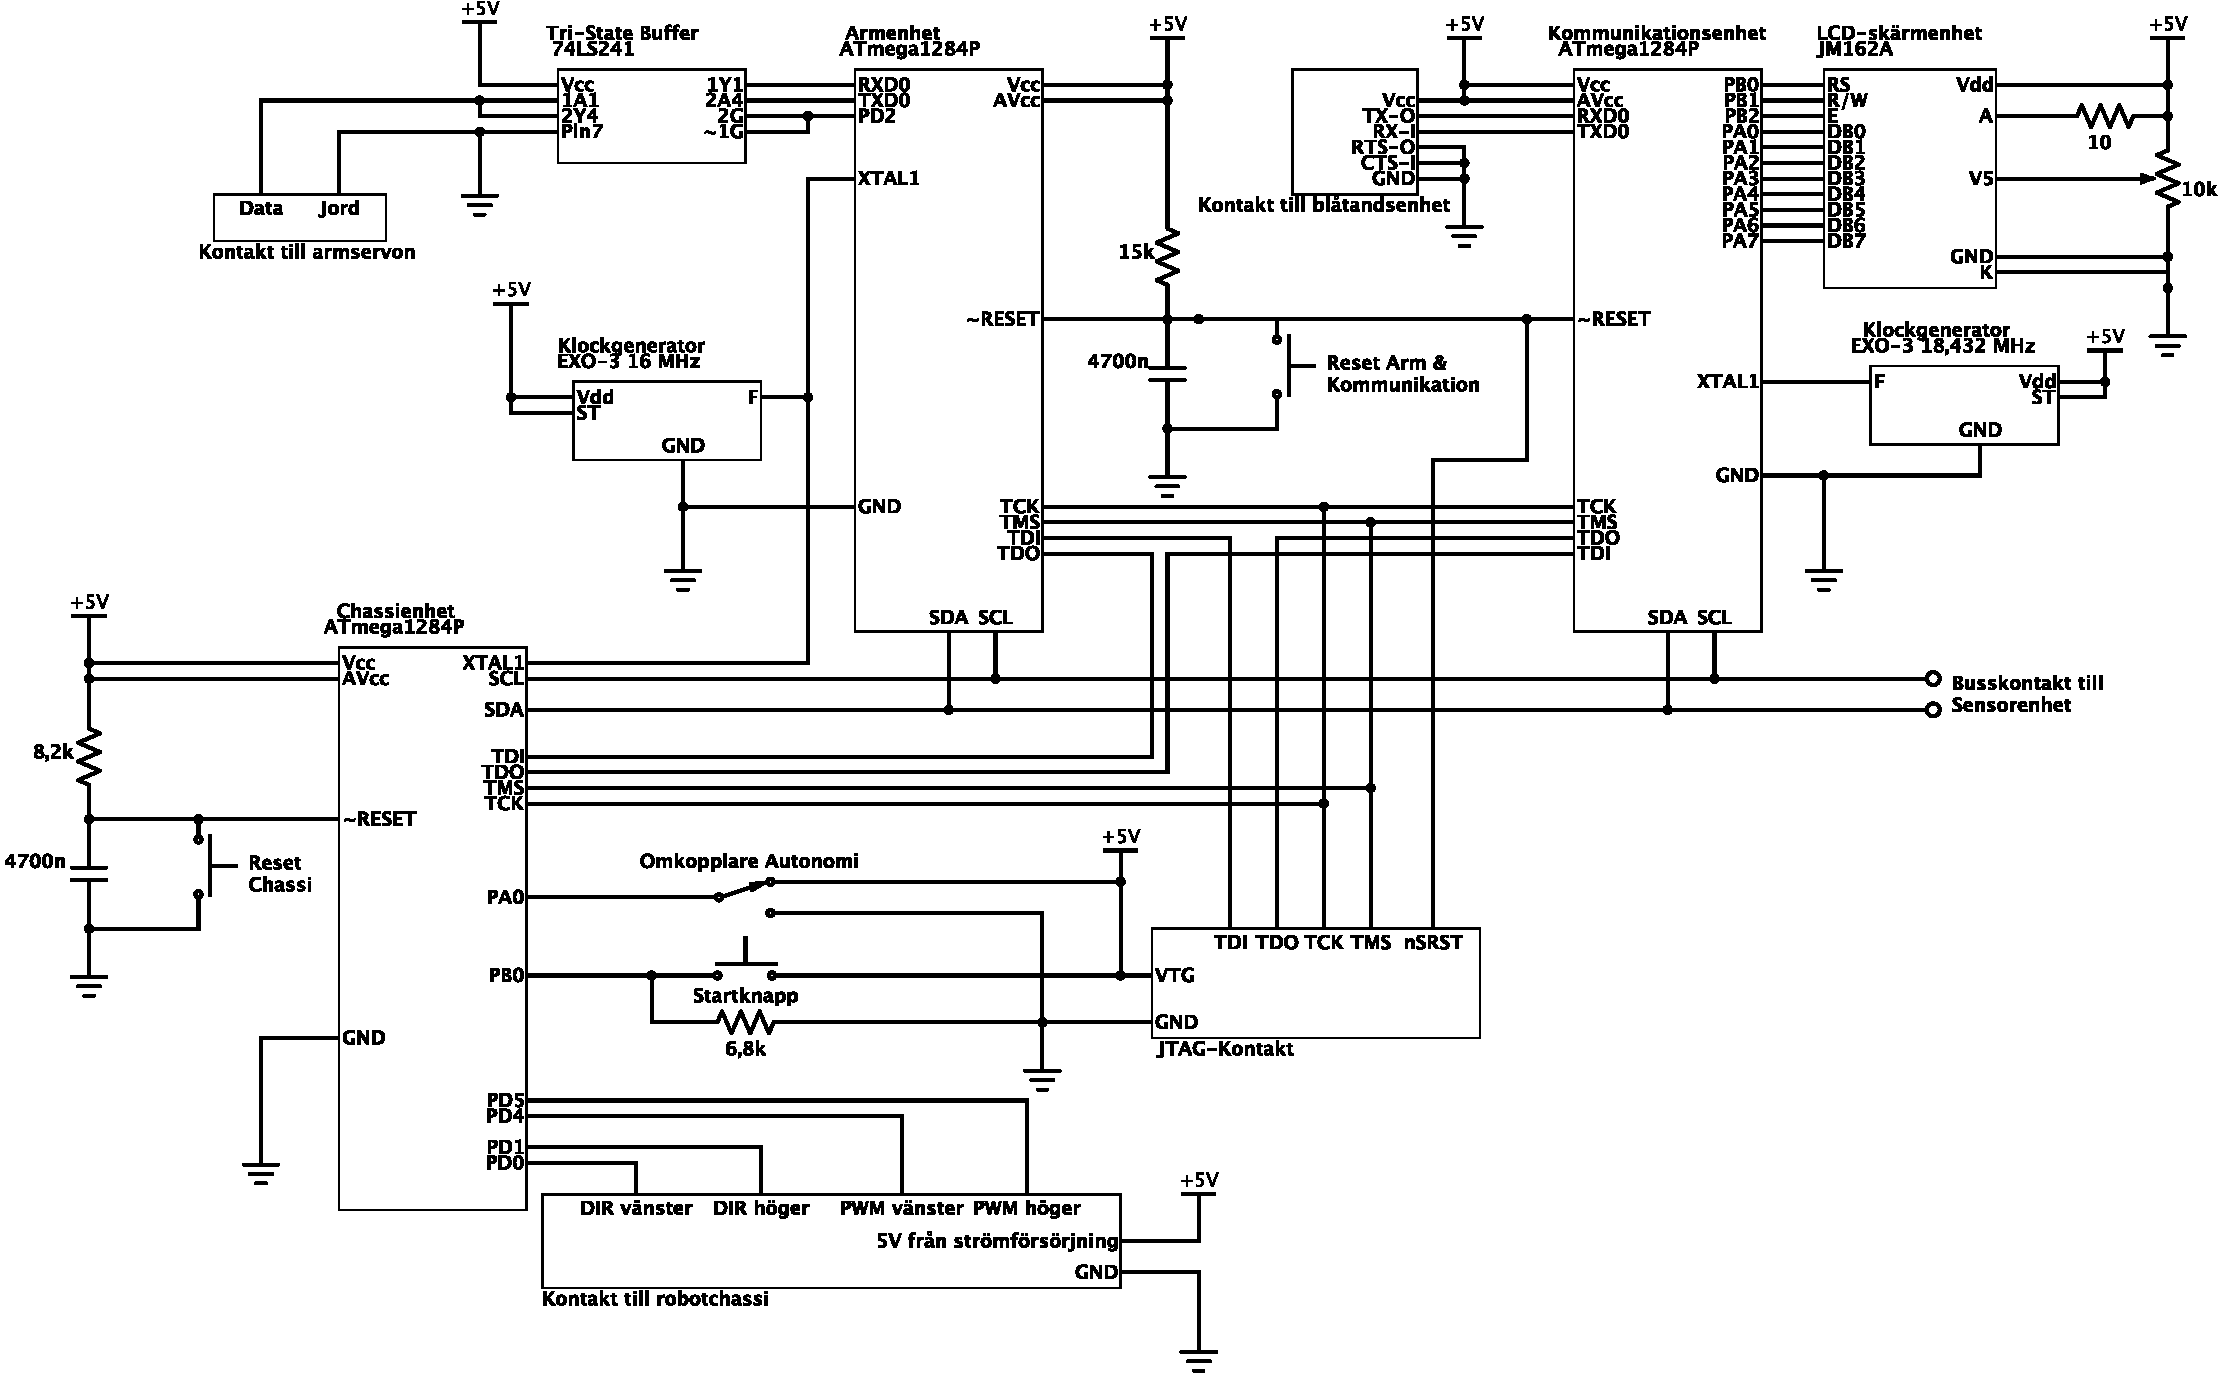
\includegraphics[angle=90,width=0.9\textwidth]{bilder/chassiarmkomm.pdf}
  \emph{\caption{Kopplingsschema över virkortet som innehåller kommunikationsenheten, chassienheten och armenheten.} \label{fig:chassiarmkomm}}
  
\end{figure}


\section{Utdrag från programlistning}
\emph{(ca 5-10 sidor så att vi kan bedöma kodens läsbarhet mm.) och eventuell VHDL-kod}
\section{Övriga bilagor?}


\end{document} 
